% Sunroof-AS.tex
\begin{hcarentry}[new]{Sunroof}
\label{sunroof}
\report{Andrew Gill}%05/14
\participants{Jan Bracker}
\status{active}
\makeheader

Sunroof is a Domain Specific Language (DSL) for generating JavaScript.
It is built on top of the JS-monad, which, like the Haskell IO-monad, allows 
read and write access to external resources, but specifically JavaScript
resources. As such, Sunroof is primarily a feature-rich foreign
function API to the browser's JavaScript engine, and all the browser-specific
functionality, like HTML-based rendering, event handling, and 
drawing to the HTML5 canvas. 

Furthermore, Sunroof offers two threading models for 
building on top of JavaScript, atomic and blocking threads.
This allows full access to JavaScript APIs, but
using Haskell concurrency abstractions, like MVars and Channels.
In combination with the push mechanism Kansas-Comet,
Sunroof offers a great platform to build interactive web applications,
giving the ability to interleave Haskell and JavaScript computations
with each other as needed.

%**<img width=500 src="./Sunroof-Examples.png">
%*ignore
\begin{center}
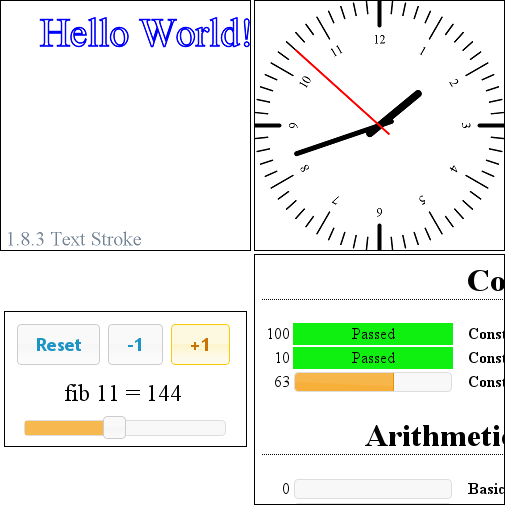
\includegraphics[width=0.35\textwidth]{html/Sunroof-Examples.png}
\end{center}
%*endignore

It has successfully been used to write smaller applications. These
applications range from 2D rendering using the HTML5 canvas element,
over small GUIs, up to executing the QuickCheck tests of Sunroof 
and displaying the results in a neat fashion.
%
The development has been active over the past 6 months and there is
a drafted paper submitted to TFP 2013.

\FurtherReading
\begin{compactitem}
\item Homepage: \url{http://www.ittc.ku.edu/csdl/fpg/software/sunroof.html}
\item Tutorial: \url{https://github.com/ku-fpg/sunroof-compiler/wiki/Tutorial}
\item Main Repository: \url{https://github.com/ku-fpg/sunroof-compiler}
\end{compactitem}
\end{hcarentry}
